\chapter{SOC model}
\label{ch:SOC}
\taskID{15}{sandpile model for self-organized criticality}

\section{Dynamical model for self-organization}
 The Bak–Tang–Wiesenfeld sandpile model is a simple example of a complex system leading to the so-called \emph{self-organizing criticality}, where large systems with many interacting components evolve toward a critical state in which even minor events can trigger significant changes, like an avalanche \cite{bak1987self}. \\
 This model is operationally defined on top of a network (originally a lattice) where each node $i$ is assigned to a critical load $t_i$. This threshold can be uniform, drawn by a particular distribution, or set to be equal to the degree of each node ($t_i=k_i$). The height $z_i$ of each site is initialized to zero. At each time step, the load by a uniformly random chosen node is increased by a unit ($z_i \to z_i+1$), changing the state of the system. A state is said to be \emph{unstable} if at least one node has height $z_i$ strictly greater than $t_i$. When this happens, all the grains at the node topple to the neighbors ($z_i \to 0$ and $z_j \to z_j + 1 \quad \forall j \in \mathcal{N}_i$), possibly causing a chain of toppling events, i.e. an \emph{avalanche} \footnote{In practice, there are different ways to model the sequential update of the states during an avalanche. In my simulations, I used a first-in-first-out queue.}. This model requires some \emph{boundary conditions} that resemble the open boundaries of a regular lattice. Thus, either $N_b$ nodes are selected as boundaries and dissipate the load, or a fraction $f$ of the grains is lost at each iteration. \\
 After a transient period, one can measure the following quantities \cite{goh2003sandpile}: (a) the number $A$ of distinct sites participating in the toppling event, i.e. the avalanche area, (b) the total number of toppling event $S$, (c) the number of toppled grains $G$, and (d) the duration $T$ of a given avalanche. In large enough networks, $A$ is equal to $S$ due to the lack of loops. \\
 The main feature of this model is the emergence of a power law with an exponential cutoff in the avalanche size distribution: $p_a(s) \sim s^{-\tau}\text{exp}(-s/s_c)$, where $s$ is the avalanche size and $s_c$ the characteristic size. The exponent $\tau$ depends on the type of the network. It has been shown that $\tau \approx 1.5$ for ER network \cite{bonabeau1995sandpile}, consistently with the mean-field solution in Euclidian space \cite{alstrom1988mean}. Since they are everywhere in nature, it is also interesting to study what happens in SF networks, i.e. networks with power-law degree distribution $p_d(k)\sim k^{-\gamma}$. In this case the expected exponent $\tau$ is related to $\gamma$ as $\tau = \gamma/(\gamma - 1)$ for $2<\gamma<3$ \cite{goh2003sandpile}. For $\gamma > 3$ one recovers the mean-field solution.  \\
 Another interesting case study is interdependent networks, e.g. $z_a-z_b$ regular graphs coupled by Bernoulli-distributed coupling studied by Brummitt et al. \cite{brummitt2012suppressing}. In the case of two independent networks $a$ and $b$, one can investigate the sizes of avalanches in $a$ caused by an initial topple in $a$ or $b$, namely $S_{aa}$ and $S_{ba}$. It has been shown that increasing interconnectivity $p$ suppresses large local cascades for small $p$ and amplifies them for large $p$. Also, tuning the interdependence to suppress cascades of a certain range leads to increased events in other ranges. This research has important consequences in many real-world networks that have a modular structure. It would be interesting to study other types of interconnectivity, for instance, in the SBM ensemble. The result of some simulations can be found in the supplementary material \ref{ch:SM_SOC2}.

\section{Numerical simulations}
The following numerical simulation compares the sandpile dynamics on top of $8$ networks with $10^4$ nodes each. The networks are generated with the \texttt{NetworkX} Python package \cite{NetworkX}. In particular, two of them are Erdős–Rényi networks ($p=7\times 10^{-4}$ and $p=2\times 10^{-3}$), and two are Barabasi-Albert networks ($m=1$ and $m=5$). Four of them are undirected scale-free networks obtained varying the $(\alpha, \beta, \gamma)$ parameters in the \texttt{scale\_free\_graph()} function to obtain different values of the power-law exponent $\gamma$. The simulations last for $10^7$ iterations with a dissipation rate of $f=1/N$. This work's main limitations are the network size and the number of simulations. 

\begin{figure}[h] 
    \centering
    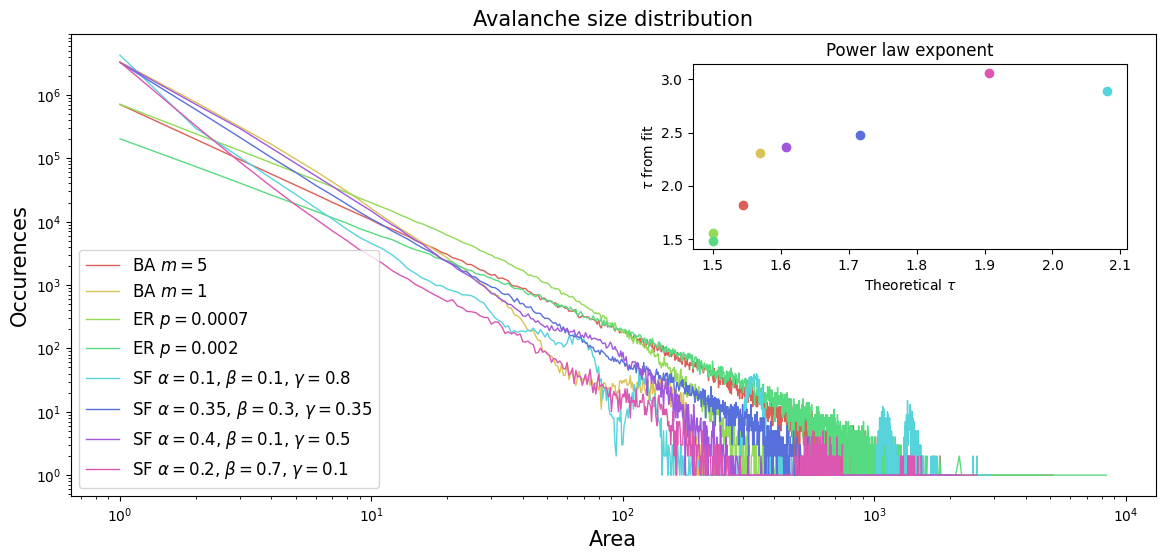
\includegraphics[width=\textwidth]{images/task15/a_dist.png} 
    \vspace{-1cm}
    \caption{(main) Power-law distributed avalanche sizes for eight different networks of $N=10^4$ nodes. Simulations of $10^7$ iterations with a dissipation rate $f=1/N$. (inset) Comparison between the exponent $\tau$ expected from the properties of the network and the one obtained by fitting the curves.}
    \label{fig:adist} 
\end{figure}

\noindent To find the expected $\tau$, one must first estimate the degree exponent $\gamma$ for the scale-free networks. This already comes with statistical implications for the reliability of this analysis. For instance, a BA network with $m=1$ is expected to have $\gamma = 3$ but was estimated at $2.76$. Then, one can fit the avalanche size distribution and compute the correspondent $\tau$ from the simulations. To limit the noise of the distribution tail, the fit is done with the first $10$ points only. \\
In scale-free networks, the power-law exponent from the simulations is typically greater than the expected one. This can be related to the finite-size effects of this analysis, leading to curves with higher slopes and faster decay. To improve the agreement, one should run longer simulations in larger networks. \\
Other figures can be found in the supplementary material \ref{ch:SM_SOC} and \ref{ch:SM_SOC2}.

 